\documentclass{standalone}
\usepackage{xcolor}
\usepackage{verbatim}
\usepackage[T1]{fontenc}
\usepackage{graphics}
\usepackage{hyperref}
\newcommand{\code}[1]{\texttt{#1}}
\newcommand{\R}{R}
\newcommand{\pkg}[1]{#1}
\newcommand{\CRANpkg}[1]{\pkg{#1}}%
\newcommand{\BIOpkg}[1]{\pkg{#1}}
\usepackage{amsmath,amssymb,array}
\usepackage{booktabs}
\usepackage{multicol, calc}
\usepackage{tikz}
\usetikzlibrary{patterns,positioning,babel}
\usepackage{threeparttable}
\usepackage{natbib}
\usepackage{inconsolata}
\usepackage{listings}
\usepackage{tikz-qtree}
\usepackage{subcaption} 

\begin{document}
\nopagecolor
	
		
		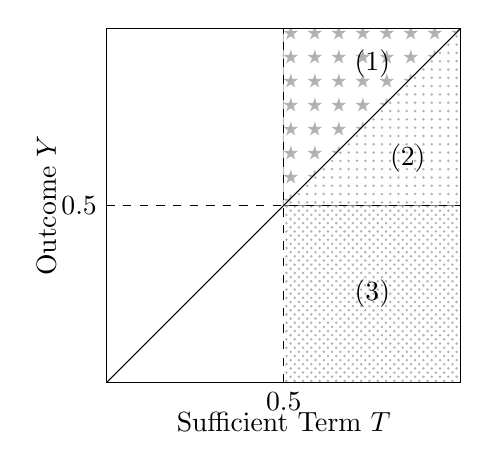
\begin{tikzpicture}[scale=4.5]
		\draw[black] (0,0) -- (1,0) node at (0.5,-0.11){Sufficient Term $T$};
		\draw[black] (0,0) -- (0,1) node at (-0.17,0.5)[rotate=90] {Outcome $Y$};
		\draw[black] (0,0) -- (1,1);
		\draw[black] (0,1) -- (1,1);
		\draw[black] (1,0) -- (1,1);
		\draw[dashed] (0.5,0) -- (0.5, 1);
		\draw[dashed] (0,0.5) -- (1, 0.5);
		\node [below] at (0.5,0){$0.5$};
		\node [left] at (0,0.5){$0.5$};
		%\draw[fill=red, opacity=0.5] (0.5,0.5) -- (0.5,0.5) -- (0.5,1) -- (1,1);
		\draw[pattern=fivepointed stars, pattern color=black, opacity=0.3] (0.5,0.5) -- (0.5,0.5) -- (0.5,1) -- (1,1);
		\node at (0.75,0.9) {(1)};
		\draw[pattern=dots, opacity=0.3] (0.5,0.5) -- (1,0.5) -- (1,1);
		\node[below] at (0.85, 0.7) {(2)};
		\draw[pattern=crosshatch dots, opacity=0.3] (0.5,0) -- (1,0) -- (1,0.5) -- (0.5,0.5);
		\node at (0.75,0.25){(3)};
		\end{tikzpicture}
		\qquad
		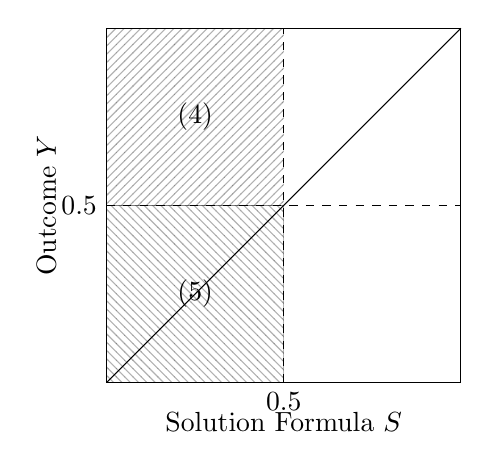
\begin{tikzpicture}[scale=4.5]
		\draw[black] (0,0) -- (1,0) node at (0.5,-0.11){Solution Formula $S$};
		\draw[black] (0,0) -- (0,1) node at (-0.17,0.5)[rotate=90] {Outcome $Y$};
		\draw[black] (0,0) -- (1,1);
		\draw[black] (0,1) -- (1,1);
		\draw[black] (1,0) -- (1,1);
		\draw[dashed] (0.5,0) -- (0.5, 1);
		\draw[dashed] (0,0.5) -- (1, 0.5);
		\node [below] at (0.5,0){$0.5$};
		\node [left] at (0,0.5){$0.5$};
		\draw[pattern=north east lines, opacity=0.3] (0.5,0.5) -- (0,0.5) -- (0,1) -- (0.5,1);
		\node at (0.25, 0.75) {(4)};
		\draw[pattern=north west lines, opacity=0.3] (0,0) -- (0,0.5) -- (0.5,0.5) -- (0.5,0);
		\node at (0.25, 0.25) {(5)};
		\end{tikzpicture}
\end{document}
